\documentclass[brazil]{beamer}
\usepackage{beamerthemesplit}
\usepackage[brazilian]{babel}
\usepackage[utf8]{inputenc}
\usepackage{color}
\usepackage{xcolor}
\usepackage{graphicx}
%\usepackage{subcaption}
\usepackage{float}
\usepackage{wrapfig}
\usepackage{amssymb}
\usepackage{amsmath}
\usepackage{fancybox}
\usepackage{ulem}
\usepackage{listings}
\usepackage{upquote}
\usetheme{JuanLesPins}
%\usetheme{Warsaw}
%\usetheme{CambridgeUS}
%\usetheme{Malmoe}


%\newcommand{\lyxline}[1][1pt]{%
%  \par\noindent%
%  \rule[.5ex]{\linewidth}{#1}\par}


\title{
  Projeto Ouroboros
}
\subtitle{
  Um sistema de integração automatizada entre C++ e
  linguagens de script
}
\author{Wilson Kazuo Mizutani e Fernando Omar Aluani}

\begin{document}

% ---------------------------------------------------------------------------- %
% Opções de listing usados para o código fonte
% Ref: http://en.wikibooks.org/wiki/LaTeX/Packages/Listings
\lstdefinelanguage{lua}
  {morekeywords={and,break,do,else,elseif,end,false,for,function,if,in,local,
     nil,not,or,repeat,return,then,true,until,while},
   morekeywords={[2]arg,assert,collectgarbage,dofile,error,_G,getfenv,
     getmetatable,ipairs,load,loadfile,loadstring,next,pairs,pcall,print,
     rawequal,rawget,rawset,select,setfenv,setmetatable,tonumber,tostring,
     type,unpack,_VERSION,xpcall},
   morekeywords={[2]coroutine.create,coroutine.resume,coroutine.running,
     coroutine.status,coroutine.wrap,coroutine.yield},
   morekeywords={[2]module,require,package.cpath,package.load,package.loaded,
     package.loaders,package.loadlib,package.path,package.preload,
     package.seeall},
   morekeywords={[2]string.byte,string.char,string.dump,string.find,
     string.format,string.gmatch,string.gsub,string.len,string.lower,
     string.match,string.rep,string.reverse,string.sub,string.upper},
   morekeywords={[2]table.concat,table.insert,table.maxn,table.remove,
   table.sort},
   morekeywords={[2]math.abs,math.acos,math.asin,math.atan,math.atan2,
     math.ceil,math.cos,math.cosh,math.deg,math.exp,math.floor,math.fmod,
     math.frexp,math.huge,math.ldexp,math.log,math.log10,math.max,math.min,
     math.modf,math.pi,math.pow,math.rad,math.random,math.randomseed,math.sin,
     math.sinh,math.sqrt,math.tan,math.tanh},
   morekeywords={[2]io.close,io.flush,io.input,io.lines,io.open,io.output,
     io.popen,io.read,io.tmpfile,io.type,io.write,file:close,file:flush,
     file:lines,file:read,file:seek,file:setvbuf,file:write},
   morekeywords={[2]os.clock,os.date,os.difftime,os.execute,os.exit,os.getenv,
     os.remove,os.rename,os.setlocale,os.time,os.tmpname},
   alsodigit = {.},
   sensitive=true,
   morecomment=[l]{--},
   morecomment=[s]{--[[}{]]},
   morestring=[b]",
   morestring=[d]',
   morestring=[s]{[[}{]]},
  }

\lstset{ %
  language=C++,                     % choose the language of the code
  basicstyle=\ttfamily\scriptsize,  % the size of the fonts that are used for the code
  numbers=left,                     % where to put the line-numbers
  numberstyle=\footnotesize,        % the size of the fonts that are used for the line-numbers
  stepnumber=1,                     % the step between two line-numbers. If it's 1 each line will be numbered
  numbersep=5pt,                    % how far the line-numbers are from the code
  showspaces=false,                 % show spaces adding particular underscores
  showstringspaces=false,           % underline spaces within strings
  showtabs=false,                   % show tabs within strings adding particular underscores
  %frame=single,                     % adds a frame around the code
  %framerule=0.6pt,
  tabsize=2,                        % sets default tabsize to 2 spaces
  captionpos=b,                     % sets the caption-position to bottom
  breaklines=true,                  % sets automatic line breaking
  breakatwhitespace=false,          % sets if automatic breaks should only happen at whitespace
  escapeinside={\%*}{*)},           % if you want to add a comment within your code
  %backgroundcolor=\color[rgb]{1.0,1.0,1.0}, % choose the background color.
  %rulecolor=\color[rgb]{0.8,0.8,0.8},
  basicstyle=\ttfamily\scriptsize,
  keywordstyle=\color{blue}\bfseries,
  keywordstyle=[2]\color[rgb]{.4,0,.4}\bfseries,
  commentstyle=\color[rgb]{0,.6,0},
  stringstyle=\color{red},
  showstringspaces=false,
  upquote=true,
  extendedchars=true,
  %xleftmargin=10pt,
  %xrightmargin=10pt,
  %framexleftmargin=10pt,
  %framexrightmargin=10pt,
  morekeywords={[2]include,ifdef,define,ifndef,endif,}
}

\frame{\titlepage}

\frame{\tableofcontents}

%-------------------------------------
\section{Introdução: Motivações e Objetivos}
%-------------------------------------
\frame{
  \begin{center}
  \LARGE 1. Introdução: Motivações e Objetivos
  \end{center}
}
%-------------------------------------
\begin{frame}[fragile]
  \frametitle{Sistema de \textit{scripts} da UGDK}
  \pause
  \begin{figure}
    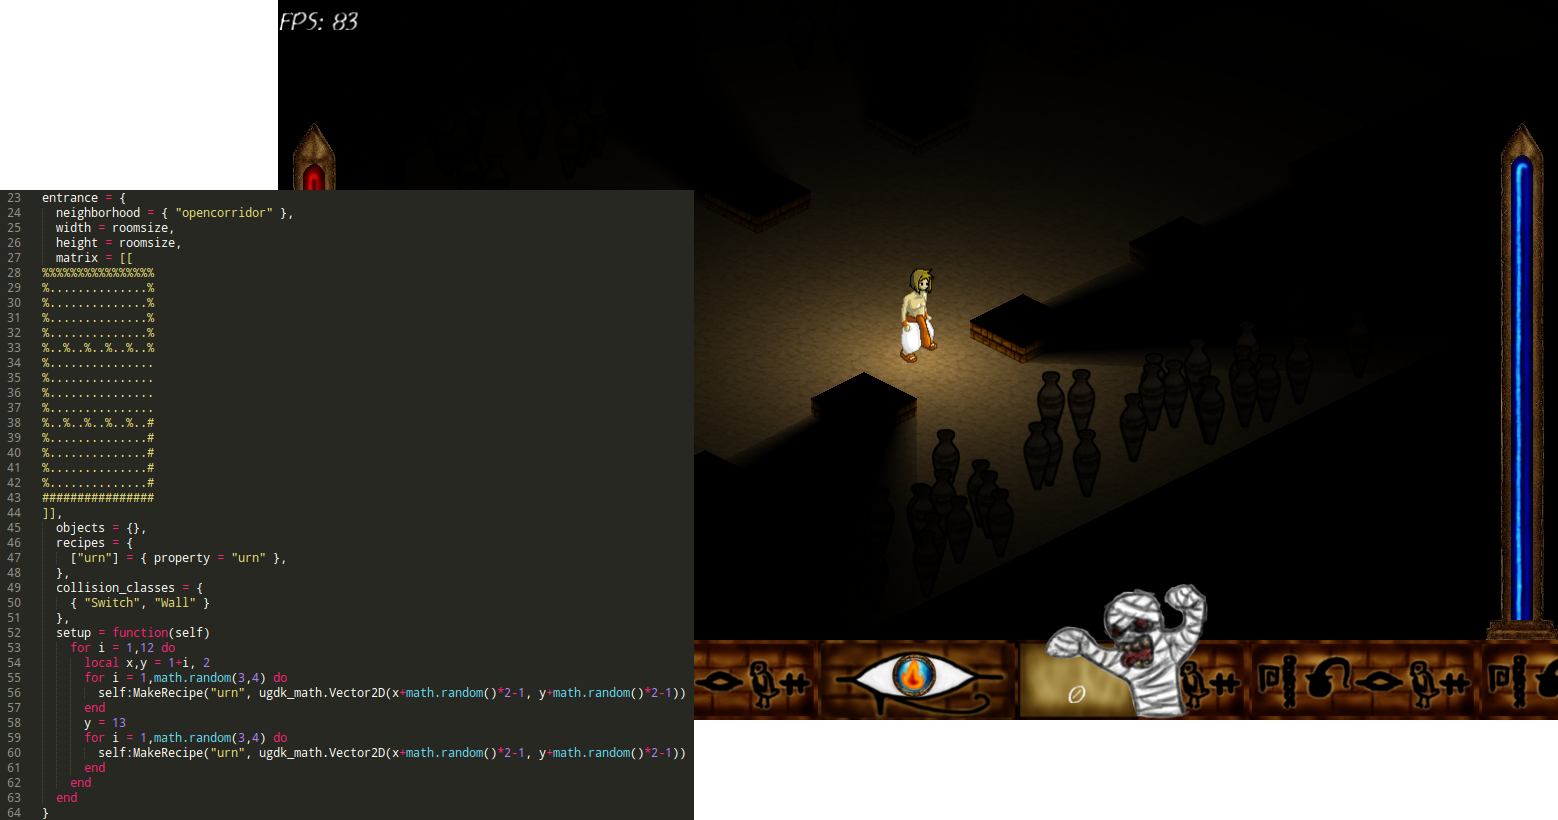
\includegraphics[width=.8\textwidth]{images/horus+sublime.png}
  \end{figure}
  \vspace{-10pt}
  \begin{itemize}
    \pause
    \item Interface única para diferentes linguagens de script
    \pause
    \item Exportação automatizada das classes em C++ (via SWIG).
  \end{itemize}
\end{frame}
%-------------------------------------
\frame{
  \frametitle{Proposta de TCC}
  \pause
  \vspace{-20pt}
  \begin{center}
    Projeto Ouroboros
  \end{center}
  \vspace{20pt}
  \begin{itemize}
    \pause
    \item Resolver os problemas do SWIG
    \vspace{10pt}
    \pause
    \item Independência da UGDK
    \vspace{10pt}
    \pause
    \item Software Livre
  \end{itemize}
}
%-------------------------------------
\section{Alguns Conceitos}
%-------------------------------------
\frame{
  \begin{center}
  \LARGE 2. Alguns Conceitos
  \end{center}
}
%-------------------------------------
\begin{frame}[fragile]
  \frametitle{Linguagens de programação}
  \pause
  Segundo Anthony A. Aaby:
  \pause
  \vspace{2em}
  \begin{block}{}
    Programas \textbf{especificam uma computação} e as notações usadas para
    descrevê-los são ditas \textbf{linguagens de programação}. [1]
  \end{block}
  \pause
  \vspace{2em}
  \begin{center}
    Então o que quer dizer ``linguagem de \textit{script}''?
  \end{center}
\end{frame}
%-------------------------------------
\begin{frame}[fragile]
  \frametitle{Linguagens de \textit{script}}
  \pause
  \begin{center}
    \LARGE
    Compilação vs. Interpretação
  \end{center}
  \pause
  \begin{figure}
    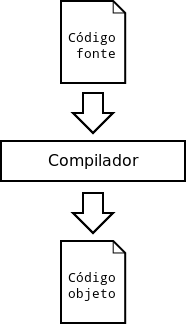
\includegraphics[width=.2\textwidth]{images/compilador.png}
    \hspace{5em}
    \pause
    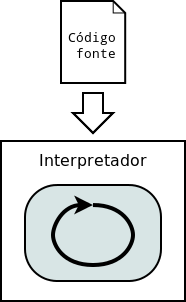
\includegraphics[width=.2\textwidth]{images/interpretador.png}
  \end{figure}
\end{frame}
%-------------------------------------
\begin{frame}[fragile]
  \frametitle{Máquinas virtuais}
  %\pause
  %\begin{center}
  %  Linguagem Nativa vs. Linguagem Virtual
  %\end{center}
  \pause
  \begin{figure}
    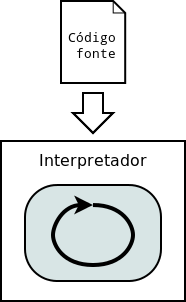
\includegraphics[height=.5\textheight]{images/interpretador.png}
  \end{figure}
\end{frame}
%-------------------------------------
\begin{frame}[fragile]
  \frametitle{Máquinas virtuais}
  \begin{figure}
    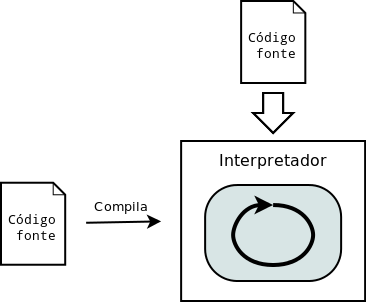
\includegraphics[height=.5\textheight]{images/nativo-vs-virtual-01.png}
  \end{figure}
\end{frame}
%-------------------------------------
\begin{frame}[fragile]
  \frametitle{Máquinas virtuais}
  \begin{figure}
    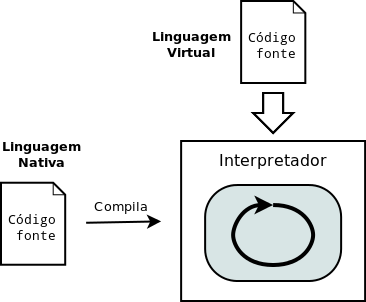
\includegraphics[height=.5\textheight]{images/nativo-vs-virtual-02.png}
  \end{figure}
\end{frame}
%-------------------------------------
\begin{frame}[fragile]
  \frametitle{Máquinas virtuais}
  \begin{figure}
    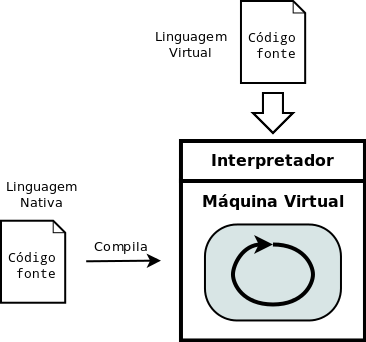
\includegraphics[height=.6\textheight]{images/nativo-vs-virtual-03.png}
  \end{figure}
\end{frame}
%-------------------------------------
\begin{frame}[fragile]
  \frametitle{Máquinas virtuais}
  \begin{figure}
    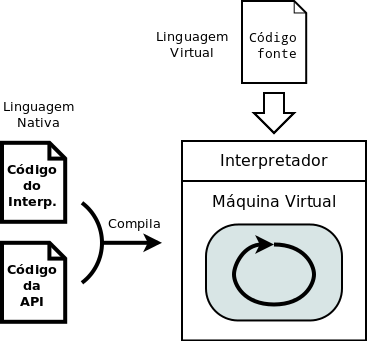
\includegraphics[height=.6\textheight]{images/nativo-vs-virtual-04.png}
  \end{figure}
\end{frame}
%-------------------------------------
\begin{frame}[fragile]
  \frametitle{Exercício 1.1: Hello World!!!}
  \pause
  \begin{columns}
    \column[t]{.5\textwidth}
      \begin{block}{helloworld.lua}
        \begin{lstlisting}
// My hello world C++ program:
printf("Hello World!");
        \end{lstlisting}
      \end{block}
    \pause
    \column[t]{.5\textwidth}
      \begin{block}{Saída}
        \begin{lstlisting}[language=lua]
-- My hello world Lua program
print "Hello World"
        \end{lstlisting}
      \end{block}
  \end{columns}
\end{frame}
%-------------------------------------
\subsection{2.1. Tipos escalares.}
%-------------------------------------
\frame{
  \begin{center}
  \Large 2.1. Tipos escalares
  \end{center}
}
%-------------------------------------
\frame{
  \frametitle{Tipagem Dinâmica}
  \begin{itemize}
    \pause
    \item Comum em linguagens de script.
    \pause
    \item O tipo de uma variável é definido pelo valor atual dela.
    \pause
    \item Portanto, o tipo de uma variável pode mudar ao longo do
          programa.
  \end{itemize}
}
%-------------------------------------
\subsection{2.2. Operações básicas}
%-------------------------------------
\frame{
  \begin{center}
  \Large 2.2. Operações básicas
  \end{center}
}
%-------------------------------------
%% TODO: exercício
\frame{
  \frametitle{Exercício 2.1}
}
%-------------------------------------
\section{Expressões de controle}
%-------------------------------------
\frame{
  \begin{center}
  \LARGE 3. Expressões de controle
  \end{center}
}
%-------------------------------------
\subsection{3.1. Estruturas}
%-------------------------------------
\frame{
  \begin{center}
  \Large 3.1. Estruturas
  \end{center}
}
%-------------------------------------
%% TODO: exercício
\frame{
  \frametitle{Exercício 3.1}
}
%-------------------------------------
%% TODO: exercício
%% sugestão: fazer um mesmo loop usando while, repeat e for.
\frame{
  \frametitle{Exercício 3.2}
}
%-------------------------------------
\subsection{3.2. Escopo.}
%-------------------------------------
\frame{
  \begin{center}
  \Large 3.2. Escopo
  \end{center}
}
%-------------------------------------
\frame{
  \frametitle{Blocos}
  \begin{itemize}
    \pause
    \item Um script lua apresenta uma hierarquia de blocos.
    \pause
    \item Um bloco é uma sequência de comandos, como os
          exemplos que vimos até agora.
    \pause
    \item Um bloco pode ter outros blocos dentro de si,
          através de:
    \begin{itemize}
      \pause
      \item estruturas de controle (if, while, for, etc);
      \pause
      \item definições de funções; ou
      \pause
      \item uso explícito de "do..end".
    \end{itemize}
  \end{itemize}
}
%-------------------------------------
\frame{
  \frametitle{Visibilidade}
  \begin{itemize}
    \pause
    \item Variáveis globais são visíveis a partir de
          qualquer bloco, contanto que não esteja
          obscurecida por alguma variável local visível
          de mesmo nome.
    \pause
    \item Variáveis locais são visíveis no bloco em que
          foram declaradas e nos blocos aninhados nele,
          contanto que sejam referenciadas após a linha em
          que foram definidas.
    \pause
    \item Se um bloco tenta acessar uma variável que não
          está visível de jeito nenhum para ele, ele
          receberá um 'nil'.
  \end{itemize}
}
%-------------------------------------
%% TODO: exercício "o i do for é global ou local?"
\frame{
  \frametitle{Exercício 3.3}
}
%-------------------------------------
\section{Funções}
%-------------------------------------
\frame{
  \begin{center}
  \LARGE 4. Funções
  \end{center}
}
%-------------------------------------
\subsection{4.1. Criando e usando funções}
%-------------------------------------
\frame{
  \begin{center}
  \Large 4.1. Criando e usando funções
  \end{center}
}
%-------------------------------------
%% TODO exercício
\frame{
  \frametitle{Exercício 4.1}
}
%-------------------------------------
%% TODO exercício
\frame{
  \frametitle{Exercício 4.2}
}
%-------------------------------------
\subsection{4.2. Upvalues}
%-------------------------------------
\frame{
  \begin{center}
  \Large 4.2. Upvalues
  \end{center}
}
%-------------------------------------
%% TODO exercício
%% - a variável "upvalue" era necessária?
\frame{
  \frametitle{Exercício 4.3}
}
%-------------------------------------
\section{Tabelas}
%-------------------------------------
\frame{
  \begin{center}
  \LARGE 5. Tabelas
  \end{center}
}
%-------------------------------------
\subsection{5.1. Criando e manipulando tabelas}
%-------------------------------------
\frame{
  \begin{center}
  \Large 5.1. Criando e manipulando tabelas
  \end{center}
}
%-------------------------------------
%% TODO: exercício
\frame{
  \frametitle{Exercício 5.1}
}
%-------------------------------------
%% TODO: exercício
\frame{
  \frametitle{Exercício 5.2}
}
%% - sugestão: construir "tabuada"
%-------------------------------------
%% TODO: exercício
\frame{
  \frametitle{Exercício 5.3}
}
%% - desafio: qual a diferença entre
%%   usar pairs e usar foreach?
%-------------------------------------
%% TODO exercício
\frame{
  \frametitle{Exercício 5.4}
}
%-------------------------------------
\begin{frame}[fragile]
  \frametitle{Possibilidades e restrições}
  \begin{itemize}
    \pause
    \item Praticamente QUALQUER COISA pode ser inserido em uma
          tabela de Lua, seja como chave ou como valor.
    \pause
    \item Isso significa que tabelas podem ter outras tabelas e
          até mesmo funçoes como chaves e valores!
    \pause
    \item A ÚNICA EXCEÇÃO é o \verb$nil$:
    \begin{itemize}
      \pause
      \item Chaves NUNCA podem ser \verb$nil$ (isso causa um erro)
      \pause
      \item Campos com valores \verb$nil$ são removidos da tabela.
    \end{itemize}
  \end{itemize}
\end{frame}
%-------------------------------------
%% TODO exercício
\frame{
  \frametitle{Exercício 5.5}
}
%-------------------------------------
\subsection{5.2. Atalhos}
%-------------------------------------
\frame{
  \begin{center}
  \Large 5.2. Atalhos
  \end{center}
}
%-------------------------------------
%% TODO exercício
\frame{
  \frametitle{Exercício 5.6}
}
%-------------------------------------
\section{Bibliotecas básicas}
%-------------------------------------
\frame{
  \begin{center}
    \LARGE 6. Bibliotecas básicas
  \end{center}
}
%-------------------------------------
\begin{frame}
  \vspace{15pt}
  Em inglês: \url{http://www.lua.org/manual/5.1/}

  Em português: \url{http://www.lua.org/manual/5.1/pt/}
\end{frame}
%-------------------------------------
%% TODO exercício
\frame{
  \frametitle{Exercícios 6.*}
}
%-------------------------------------
\section{Unlimited slide works}
%-------------------------------------
\frame{
  \begin{center}
    \LARGE ENFIM...
  \end{center}
}
%-------------------------------------
\begin{frame}
  \frametitle{Tópicos avançados que não aparecem nos slides}
  \begin{itemize}
    \item Tipos thread e userdata.
    \item Bibliotecas avançadas: module. debug e thread.
    \item Ambientes de funções.
    \item Metatabelas.
    \item API C.
  \end{itemize}
\end{frame}
%-------------------------------------
\begin{frame}
  \begin{center}
    \LARGE Obrigado!
  \end{center}
  \begin{itemize}
    \item Visitem www.uspgamedev.org
    \item Dúvidas: kazuo@uspgamedev.org
    \item Se seu interesse for desenvolvimento de games,
          vale MUITO a pena dar uma conferida na engine
          LÖVE2D.
    \begin{itemize}
      \item Site oficial: www.love2d.org
      \item Jogo feito com LÖVE2D: http://stabyourself.net/mari0
    \end{itemize}
  \end{itemize}
\end{frame}
%-------------------------------------
\begin{frame}
  \frametitle{Bibliografia}
  \begin{itemize}
    \footnotesize
    \item[1]
      Anthony A. Aaby. \textit{Introduction to Programming Languages}. 1996.
      Disponível em
      \begin{center}
        \scriptsize
        \url{http://www.emu.edu.tr/aelci/Courses/D-318/D-318-Files/plbook/}

        (último acesso em 29/10/2013)
      \end{center}
  \end{itemize}
\end{frame}
%-------------------------------------
\end{document}

